\chapter{Contribution on Visual Odometry}%
\label{cha:vors}

\minitoc%

\section{RGB-D Tracking Evaluation}%
\label{sec:rgbd-tracking-evaluation}

Un dépot pour faciliter la comparaison d’algorithmes d’odométrie visuelle RGB-D. Les tests sont basés sur le dataset TUM RGB-D, ou tout dataset compatible (comme ICL-NUIM qui est un dataset synthétique). En l’état actuel des choses, des programmes de test sont prêts pour les algos suivants :
- OpenCV, en trois versions :
  - one direct approach (Rgbd) based on the paper "Real-Time Visual Odometry from Dense RGB-D Images", F. Steinbucker, J. Strum, D. Cremers, ICCV, 2011.
  - one point cload approach (ICP) based on the paper "KinectFusion: Real-Time Dense Surface Mapping and Tracking", Richard A. Newcombe, Andrew Fitzgibbon, at al, SIGGRAPH, 2011.
  - one mixed approach (RgbdICP) minimizing the sum of both energy functions.
- The fovis visual odometry library, based on the paper "Visual Odometry and Mapping for Autonomous Flight Using an RGB-D Camera", Albert S. Huang, Abraham Bachrach, Peter Henry, Michael Krainin, Daniel Maturana, Dieter Fox, and Nicholas Roy. Int. Symposium on Robotics Research (ISRR), Flagstaff, Arizona, USA, Aug. 2011
- Dense Visual Odometry (DVO), based on the paper "Robust Odometry Estimation for RGB-D Cameras", C. Kerl, J. Sturm and D. Cremers, In International Conference on Robotics and Automation (ICRA), 2013.
- Visual Odometry in Rust (vors), currently being worked on.

Pour analyser et comparer les trajectoires, j’ai fait un programme qui prends toutes les trajectoires en arguments, calcule la “rpe” (relative pose error) de translation et rotation à 1 frame d’écart, et 1 seconde d’écart, et finalement exporte tous les résultats dans un CSV contenant les champs suivants :

- sequence : le nom de la sequence vidéo, par exemple "rgbd\_dataset\_freiburg1\_floor"
- camera : l’identifiant de la caméra associée à la séquence : “fr1”
- algo : l’algorithme utilisé, par exemple “dvo”, “ocv-rgbd”, “vors”, “vors-robust”, ...
- t\_err\_rmse\_f : erreur de translation à 1 frame en mètre sur la séquence (rmse)
- t\_err\_median\_f : erreur de translation à 1 frame en mètre sur la séquence (médiane)
- r\_err\_rmse\_f : erreur de rotation à 1 frame en degrés sur la séquence (rmse)
- r\_err\_median\_f : erreur de rotation à 1 frame en degrés sur la séquence (médiane)
- t\_err\_rmse\_s : erreur de translation à 1 seconde en mètre sur la séquence (rmse)
- t\_err\_median\_s : erreur de translation à 1 seconde en mètre sur la séquence (médiane)
- r\_err\_rmse\_s : erreur de rotation à 1 seconde en degrés sur la séquence (rmse)
- r\_err\_median\_s : erreur de rotation à 1 seconde en degrés sur la séquence (médiane)

Pour explorer rapidement ces résultats, j’utilise un outil de visualisation de données nommé data-voyager [github] [online]. Les derniers résultats en date, ça donne :

\begin{figure}[ht]
	\centering
	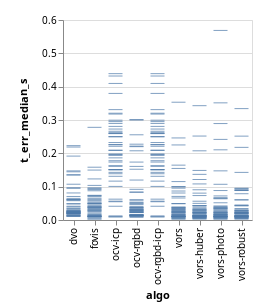
\includegraphics[width=\linewidth]{assets/img/rpe-2019-04-04.png}
	\caption{Relative pose error (rpe)}%
	\label{fig:rpe-eval}
\end{figure}

En moyenne, notre algo robuste est le meilleur. Plus d’infos sur le code d’évaluation dans le readme du dépot. Plus d’infos sur notre algo dans la section sur vors.

\section{Visual Odometry in Rust (vors)}%
\label{sec:vors}

Ce qui a démarré comme un espoir d’apporter des améliorations aux algos d’odométrie visuelle existants (en particulier DSO [github]) s’est fini en une récriture, de zéro, d’un “framework/library” d’odométrie visuelle en Rust. Les avantages techniques de Rust par rapport à C++ sont nombreux pour repartir d’une base saine mais je ne m’étends pas plus là-dessus (plus d’info dans le readme).

Le coeur d’un algo d’odométrie visuelle directe, c’est la minimisation d’une énergie de reprojection des pixels d’une image de référence à une nouvelle image. Ce problème est souvent qualifié “image alignment” par simplification dans les cas où la fonction de reprojection conserve la “topologie?” de l’image originale 2D (transformations dans le plan).

En 3D, la reprojection nécessite de connaître la profondeur d’un pixel. Le cadre le plus simple pour re-coder un algorithme de zéro, c’est donc celui du tracking caméra RGB-D (D pour depth).

Actuellement, l’algorithme implémenté dans vors est constitué des étapes suivantes :
- Générer une image multi-résolution, en teintes de gris, de l’image “keyframe”.
- Générer une image multi-résolution, en teintes de gris, de l’autre image à tracker.
- Choisir des points candidats sur le keyframe, qui vont être utilisés pour l’énergie à minimiser.
- Résoudre par un algorithme itératif (Levenberg-Marquardt) le calcul de la transformation caméra entre la keyframe et la nouvelle image :
  - Calculer le Jacobien et la Hessienne approximée (approximation de Gauss-Newton, version Levenberg-Marquardt) pour chaque résidu de l’énergie à minimiser.
  - Calculer le pas d’itération.
  - Mettre à jour la transformation caméra en compositionnel inverse
- Décider si on doit changer de keyframe.

Cette version, simple mais fonctionnelle donne d’excellents résultats sur le dataset synthétique, meilleurs que les autres algos évalués (sauf ICP). Sur le dataset réel, les résultats sont un tout petit peu en retrait comparé à DVO, fovis et OpenCV. Comme visible sur le graphique de la partie précédente, les résultats sont donc en moyenne équivalents. J’ai donc figé cette version du code, comme la version 0.1. J’en ai profité pour clarifier et documenter tout le code de cette version pour en faire une bibliothèque de l’écosystème Rust. J’y ai inclus un ensemble d’exemples d’utilisations de la lib, documentés et imagés dans le readme du dossier “examples/” du dépot.

[image] Figure représentant le processus de sélection des points candidats, qui est un des codes d’exemples.

[image] Figure représentant un exemple d’utilisation du code d’optimisation de Levenberg-Marquardt pour déterminer la transformation affine 2D entre deux images. Cet exemple sert de problème simplifié (Jacobien et Hessienne simples) pour notre problème de tracking caméra 3D. Il repose tout de même sur la même structure d’algorithme et constitue donc un excellent point d’entrée pour comprendre la version 3D caméra.

Améliorations de vors pour publications
-----

Une fois notre base vors posée. On s’est donc posé la question : “Quelles améliorations peuvent être rapidement explorées pour nous permettre d’être meilleurs que les autres algorithmes de manière consistente, y compris dans le dataset réel ?”.

Plusieurs points se sont dégagés assez rapidement, en particulier :
- Intégrer des termes photométriques dans le résidu, passer de : I\_j [ w(p) ] - I\_i [ p ]
À : a\_j * ( I\_j [ w(p) ] - b\_j )  -  a\_i * ( I\_i [ p ] - b\_i )
Ou a et b sont des termes constant dans l’image associée. Ces termes, en particulier le a permettent de prendre en compte les variations d’exposition automatiques courantes dans les séquences vidéos où l’intensité lumineuse globale de la scène varie.
- Rendre le problème de minimisation d’énergie robuste aux données aberrantes.

J’ai donc commencé en début de semaine dernière par l’amélioration avec les termes photométriques. Ça n’a pas donné ce que j’espérais. Les résultats étaient pires qu’avant. Je soupçonne que ce soit les les grands résidus (avant l’approche robuste) qui dégradent les termes photométriques plus qu’ils ne permettent d’améliorer la situation.

Je me suis donc penché en fin de semaine dernière (cf mails) sur la robustesse de la minimisation d’énergie avec deux fonctions de perte robustes :
- Huber, comme dans DSO
- Geman-McClure : x -> x\^2 / (a + x\^2)

Après rebondissements, cette fois on obtient des résultats meilleurs ! (mais pas de beaucoup)

Surtout, cette amélioration est assez sensible au choix des paramètres associés. Sachant que pour l’instant, ces paramètres sont définis globalement. J’ai été assez surpris cependant que les résultats ne soient pas meilleurs, sachant qu’ils sont environ 20\% meilleurs sur 4 des 5 datasets que j’ai testés sur mon ordinateur pendant la phase de “tuning”.

La liste des pistes d’améliorations est longue. Celle qui me semblent importantes à explorer sont les suivantes :
- Essayer une méthode statistique (déjà codée) pour construire les cartes de profondeur (semi-dense) multi-résolutions utilisées dans les itérations du problème de minimisation.
- Adapter la méthode de sélection des points candidats pour
  - 1. Améliorer la détection des points de courbures (pour l’instant on peut facilement perdre des bordures)
  - 2. Limiter le nombre de points maximum, et donc par la même occasion le rapport de densité de points entre les zones à forts et à faibles gradients. Si le rapport de densité est trop élevé, ce qui arrive assez rapidement avec beaucoup de niveaux de résolution, les points à faible gradients deviennent négligeables dans le problème de minimisation.
  - Essayer directement avec DSO aussi
- Adapter la méthode de calcul des gradients multi-résolution
  - Tester avec uniquement les gradients DSO (centrés, même résolution)
  - Tester avec des blocs 2x4 et 4x2 au lieu d’uniquement 2x2 pour ne pas “sauter” des gradients à certains niveaux de résolution.

Paramètres présents dans le code
---------------------

La multiplication du nombre de paramètres dans le code n’est pas une bonne chose. Voici donc une liste complète des paramètre réglables ayant une influence sur les performances du tracking caméra. L’objectif est de réduire ce nombre au stricte minimum.

- nb\_levels = 6 -> C’est le nombre de niveaux dans la pyramide de résolutions. En pratique, j’ai estimé (empiriquement) que 200 points à la plus faible résolution semble avoir des bons comportements. On pourrait donc déjà remplacer 6 par round( 1 + log\_4( pix / 200 ) ) pour avoir toujours environ 200 points.
- candidates\_thresh = 7 -> C’est le seuil utilisé pour la décision de prendre 2 points candidats au lieu d’un seul à la résolution supérieur lors de la sélections des candidats avec la méthode “coarse to fine”.
- max\_candidates = ? -> Ce n’est pour l’instant pas fixé, ce qui peut créer de fortes différences de densités …
- Les coefficients de Levenberg-Marquardt, (start = 0.1, multipliers = (10, 0.1) ).
- Critère d’arrêt des itérations : variation d’énergie < seuil. Ce seuil n’est pas le même suivant l’approche (robuste, …).
- Critère de changement de keyframe : optical\_flow > 1.0. J’ai essayé plusieurs valeurs pour ce critère. “Optical\_flow” est calculé comme la moyenne des déplacements des pixels entre la keyframe et l’image courante à la plus faible des résolutions de la pyramide.

Les paramètres liés aux implémentations robustes :
- Le seuil à partir duquel un résidu est abandonné (pas ajouté dans les jacobiens). Pour le moment ce seuil a donné des résultats pas trop mauvais à 50.
- Le coefficient “de coupure” correspond à l’approche robuste associée. Intuitivement, le point de bascule entre la zone convex et la zone concave de la fonction.

\subsection{Coarse to Fine Candidate Points Selection}%
\label{sub:candidates}

\subsection{Multi-Resolution Image Gradients}%
\label{sub:multires-gradients}

\subsection{Multi-Resolution Direct Image Alignment}%
\label{sub:multires-direct-image-alignment}

\subsection{Levenberg-Marquardt Optimization}%
\label{sub:lm-optimization}

\subsection{Gradients of the Reprojection Function with an Inverse Compositional Formulation}%
\label{sub:gradients-inverse-compostional}

\subsection{Robust Optimization Techniques}%
\label{sub:robust-optim}

\subsection{Photometric Term in the Residuals}%
\label{sub:photometric-residual}

